% This work is licensed under a CC0 1.0 Universal
% http://creativecommons.org/publicdomain/zero/1.0/
%
% This theme was created by Ekaterina Gerasimova <kittykat3756@gmail.com> for
% GUADEC 2013.

\documentclass{beamer}

% This work is licensed under a CC0 1.0 Universal
% http://creativecommons.org/publicdomain/zero/1.0/
%
% This theme was created by Ekaterina Gerasimova <kittykat3756@gmail.com> for
% GUADEC 2013.

\mode<presentation>
{
  \usecolortheme[RGB={203,214,218}]{structure}
  \usetheme{Frankfurt}
  \setbeamercolor{frametitle}{fg=black}
  \setbeamercolor{title}{fg=black}
  \definecolor{muddyblue}{RGB}{88,118,133}
  \setbeamercolor{section in head/foot}{fg=white, bg=muddyblue}
  \setbeamercolor{bibliography entry author}{fg=muddyblue}
  \setbeamertemplate{navigation symbols}{}

  \setbeamercovered{transparent}
	
	\parskip=\baselineskip
}

%\pgfdeclareimage[height=1cm]{guadec-logo}{guadec-logo.pdf}
%\logo{\pgfuseimage{guadec-logo}}


\usepackage[english]{babel}

\usepackage[latin1]{inputenc}

\usepackage{times}
\usepackage[T1]{fontenc}

%***********************************
%********** My packages ************
%***********************************
\usepackage[dayofweek]{datetime} 
\longdate
\usepackage{url}
%***********************************
%***********************************
%***********************************

\title[Optional short paper title]
{Applied data science capstone project \\ `The battle of neighbourhoods'}

\subtitle
{Opening an Italian resturant in London}

\author
{Francesco Bianconi \\ \href{mailto:bianco@ieee.org}{\texttt{bianco@ieee.org}}}

%\institute[University of GNOME]

\date{\today}

%Table of contents
%\AtBeginSubsection[]
%{
%  \begin{frame}<beamer>{Outline}
%    \tableofcontents[currentsection,currentsubsection]
%  \end{frame}
%}

\begin{document}

\begin{frame}
  \titlepage
\end{frame}

\section{Background and objectives}

\begin{frame}{Background}
London is the capital and largest city of England and the United Kingdom with a population of $\approx$9M

It is one of the most influential, most visited and most culturally active place in the world

Offers countless opportunities to the visitor and the residents: `\emph{When a man is tired of London, he is tired of life}' (Samuel Jackson)
\end{frame}

\begin{frame}{Objectives}
We want to open an Italian restaurant in London; the problem is to decide the most convenient place
\end{frame}

\section{Materials \& methods}

\begin{frame}[allowframebreaks]{Methodology}
We considered the town in London divided into its boroughs 

The tentative location for the new restaurant would be a generic place within one mile from the centre of the borough
\begin{center}
	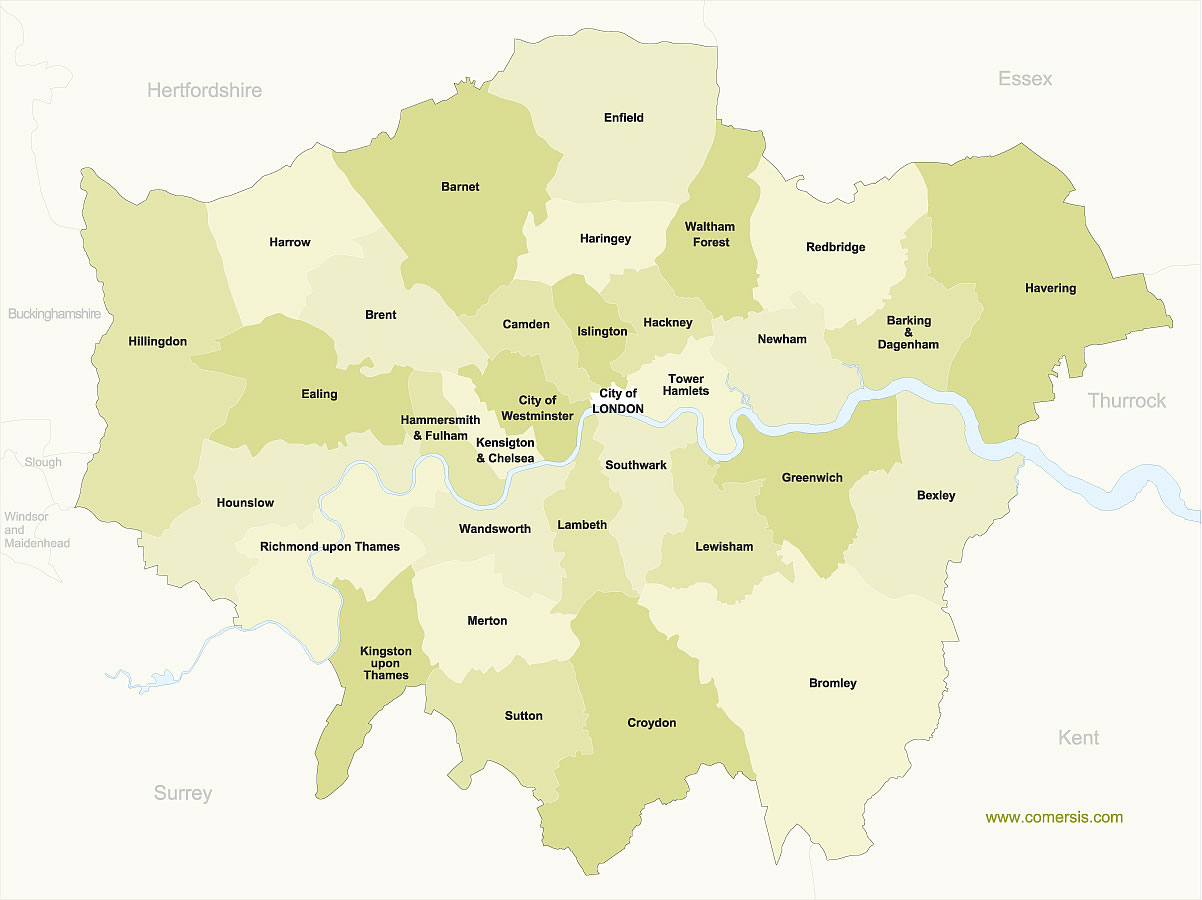
\includegraphics[width = 0.55\textwidth, keepaspectratio]{images/london-boroughs.jpg}
\end{center}

\framebreak

We compared the boroughs based on the following features:
\begin{itemize}
	\item Number of \textbf{Italian restaurants} already present (the fewer the better)
	\item Average \textbf{income} of each borough (the higher the better)
	\item \textbf{Population} of the borough (the more populated the better)
	\item Presence of amenities around like \textbf{cinemas} and \textbf{theatres} (the more the better)
	\item Presence of \textbf{universities} around (the more the better)
\end{itemize}

We ranked the boroughs by each of the above features and obtained the overall rank by averaging the results (we assumed that each feature weighed the same in determining the overall ranking) 

\end{frame}

\begin{frame}{Data sources}
We retrieved the data from the following following sites:

\begin{itemize}
	\item \url{https://en.wikipedia.org/wiki/London\_boroughs} (list of London boroughs)
	\item \url{https://data.london.gov.uk/dataset/earnings-place-residence-borough} (average income by borough, 2018)
	\item \url{https://www.citypopulation.de/en/uk/greaterlondon/} (population by borough, 2018)
\end{itemize}
\end{frame}

\begin{frame}{Data collection and analysis}
We used Python 3.7.4 and the following packages:
\begin{itemize}
  \item \href{https://python-visualization.github.io/folium/}{\underline{Folium}} for map generation
  \item \href{https://developer.foursquare.com/}{\underline{Foursquare}} to get the points of interest around the target locations
	\item \href{https://geopy.readthedocs.io/en/stable/}{\underline{GeoPy}} to retrieve the location of the centre of each borough 
	\item \href{https://pandas.pydata.org/}{\underline{Pandas}} for data collection and manipulation
\end{itemize}

All the source code is available in the \href{https://github.com/biancovic/Coursera_Capstone/blob/master/BattleOfNeighbourhoods/BattleOfNeighbourhoods.ipynb}{\underline{notebook}}
\end{frame}

\section{Results and conclusions}

\begin{frame}[allowframebreaks]{Results}
The following table shows the data arranged in a Pandas dataframe (first five rows):
\vspace{-1.5\baselineskip}
\begin{center}
	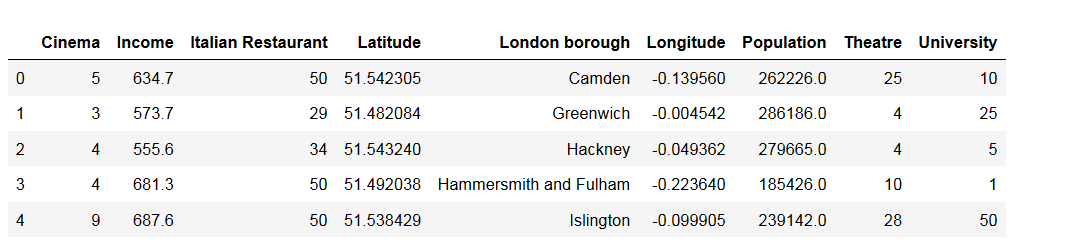
\includegraphics[width = \textwidth, keepaspectratio]{images/dataframe-snapshot-1.png}
\end{center}

And here are the data after ranking (top five results):
\vspace{-1.5\baselineskip}
\begin{center}
	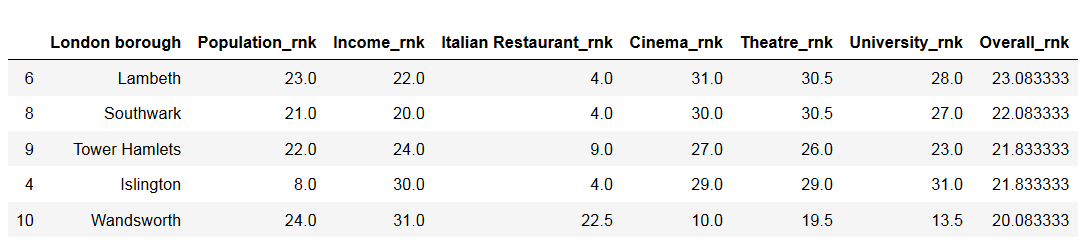
\includegraphics[width = \textwidth, keepaspectratio]{images/dataframe-snapshot-2.png}
\end{center}

\vspace{-1.0\baselineskip}

\framebreak
The picture shows the results on a map (interactive version available \href{http://biancovic.droppages.com/}{\underline{here}})

\begin{center}
	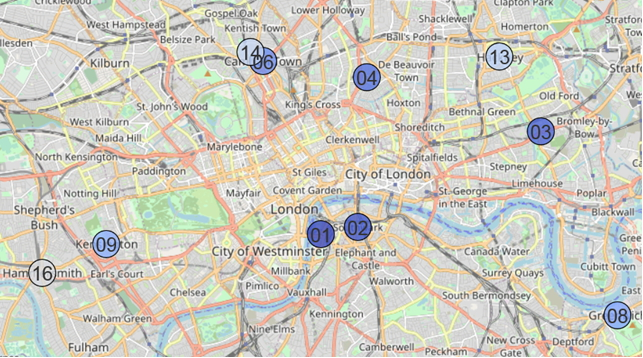
\includegraphics[width = 0.8\textwidth, keepaspectratio]{images/map.jpg}
\end{center}

\end{frame}

\begin{frame}{Conclusions}
Our study indicates that the best boroughs to open an Italian restaurant in London are (in top-down order):

\begin{itemize}
\item Lambeth (ranked $1^\text{st}$)
\item Southwark
\item Tower Hamlets
\item Islington
\item Wandsworth
\end{itemize}

Please visit the \href{https://github.com/biancovic/Coursera_Capstone/blob/master/BattleOfNeighbourhoods/BattleOfNeighbourhoods.ipynb}{\underline{notebook}} for the complete placings

\end{frame}



\end{document}
